\chapter{速度合成、光锥与四维矢量}

\section{同一条铁路轨道上的两个参考系}

此前导出的洛伦兹变换涉及一种刻意受限的几何：所有相对运动都沿一个轴。设想一条长长的铁路轨道。一组观测者留在车站；另一组观测者乘坐沿轨道行驶的列车。横向方向是存在的，但在稍后恢复它们之前，它们不起作用。

每个参考系都是一个操作性的坐标系。在参考系中静止的米尺定义空间坐标，而在参考系中静止的同步时钟定义时间。确定它们之间关系的假设是：每个惯性观测者测得相同的光速。

大多数计算将使用\(c=1\)。时间可以用秒和光秒来度量，也可以用年和光年来度量。速度于是成为光速的无量纲分数。当需要普通单位时，\(c\)的因子由量纲一致性唯一地恢复；例如，无量纲洛伦兹因子中的\(v^2\)变为\(v^2/c^2\)。

\subsection{正变换与逆变换}

设一次闪光发生在列车内或列车附近的某处。它是一个事件，与由谁描述无关。车站观测者赋予\((x,t)\)，而列车观测者赋予\((x',t')\)。在单位\(c=1\)下，
\begin{align}
x'&=\gamma_v(x-vt),&
t'&=\gamma_v(t-vx),
\label{eq:sr2-direct}\\
\gamma_v&=\frac{1}{\sqrt{1-v^2}}.
\end{align}
牛顿会认出位移\(x-vt\)；因子\(\gamma_v\)以及\(x\)混入\(t'\)则是相对论性的变化。

\begin{figure}[htbp]
\centering
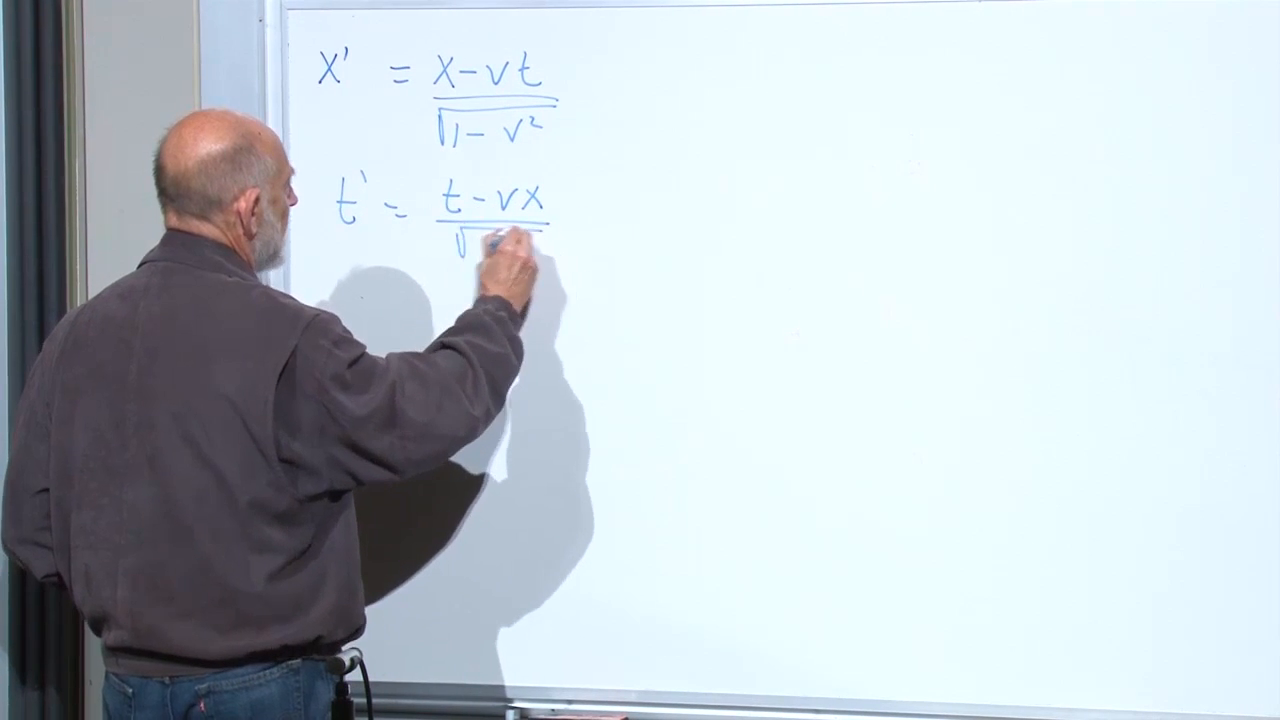
\includegraphics[width=0.90\textwidth]{lecture_02_figure_01.png}
\caption{将车站坐标\((x,t)\)与列车坐标\((x',t')\)联系起来的正洛伦兹变换。}
\lectureframe{00:07:52}
\end{figure}

互易性通过反转相对速度的符号给出逆变换：
\begin{align}
x&=\gamma_v(x'+vt'),&
t&=\gamma_v(t'+vx').
\label{eq:sr2-inverse}
\end{align}
车站并非绝对静止。它只是被称为不带撇的参考系，而列车看到它以\(-v\)运动。

\begin{figure}[htbp]
\centering
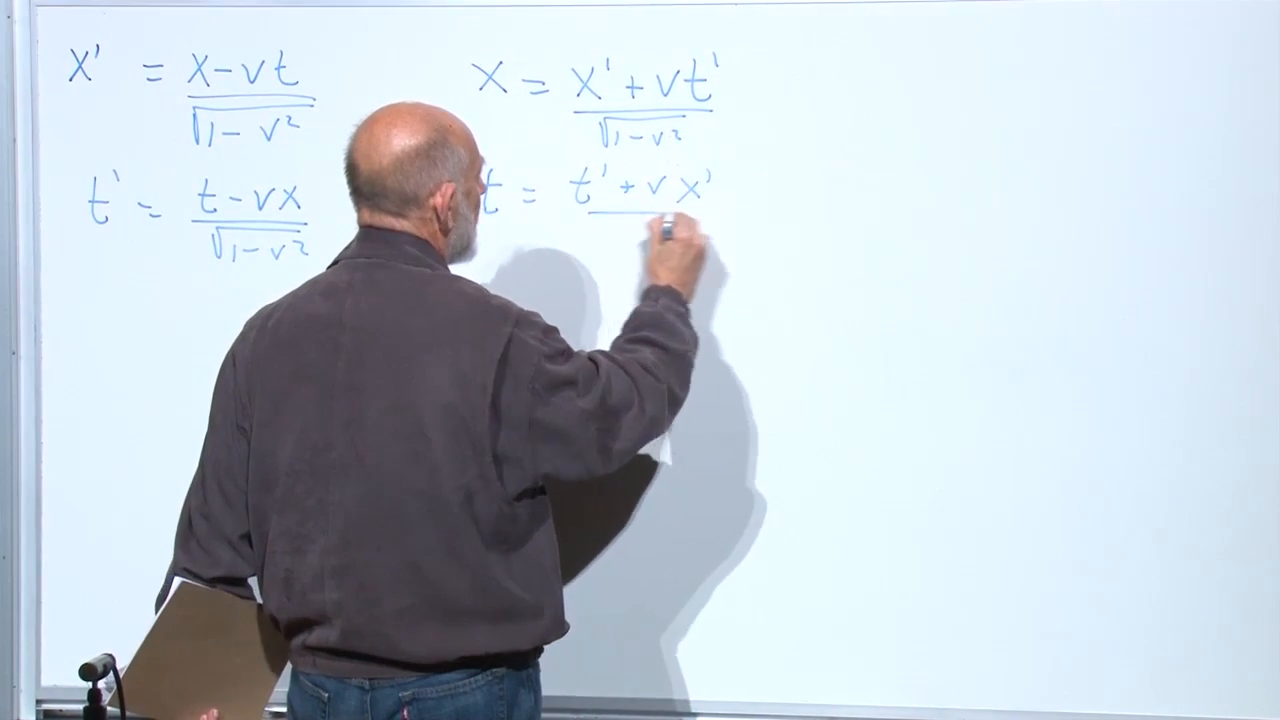
\includegraphics[width=0.90\textwidth]{lecture_02_figure_02.png}
\caption{逆映射具有相同的洛伦兹因子和相反的相对速度符号。}
\lectureframe{00:09:15}
\end{figure}

对于沿\(x\)方向的推促，横向坐标不变：
\begin{equation}
y'=y,
\qquad
z'=z.
\end{equation}

相对速率可以从空间方程读出，而无须研究其分母。列车原点由\(x'=0\)定义，因此
\begin{equation}
x'=0
\quad\Longleftrightarrow\quad
x-vt=0
\quad\Longleftrightarrow\quad
x=vt.
\label{eq:sr2-origin-worldline}
\end{equation}
这条世界线中\(t\)的系数就是列车在车站坐标中的速率。

\section{三个参考系与推促的合成}

在列车内放一辆小童车。列车相对于车站以速率\(v\)运动，而童车相对于列车乘客沿过道以速率\(u\)运动。称童车相对于车站的速率为\(w\)。牛顿式的直觉提示\(w=u+v\)，但必须由洛伦兹变换来决定。

现在有三个坐标系：
\begin{equation}
(x,t),\qquad (x',t'),\qquad (x'',t'').
\end{equation}
第一个属于车站，第二个属于列车，第三个属于童车。在列车与童车之间，
\begin{align}
x''&=\gamma_u(x'-ut'),&
t''&=\gamma_u(t'-ux'),
\label{eq:sr2-second-boost}\\
\gamma_u&=\frac{1}{\sqrt{1-u^2}}.
\end{align}

\begin{figure}[htbp]
\centering
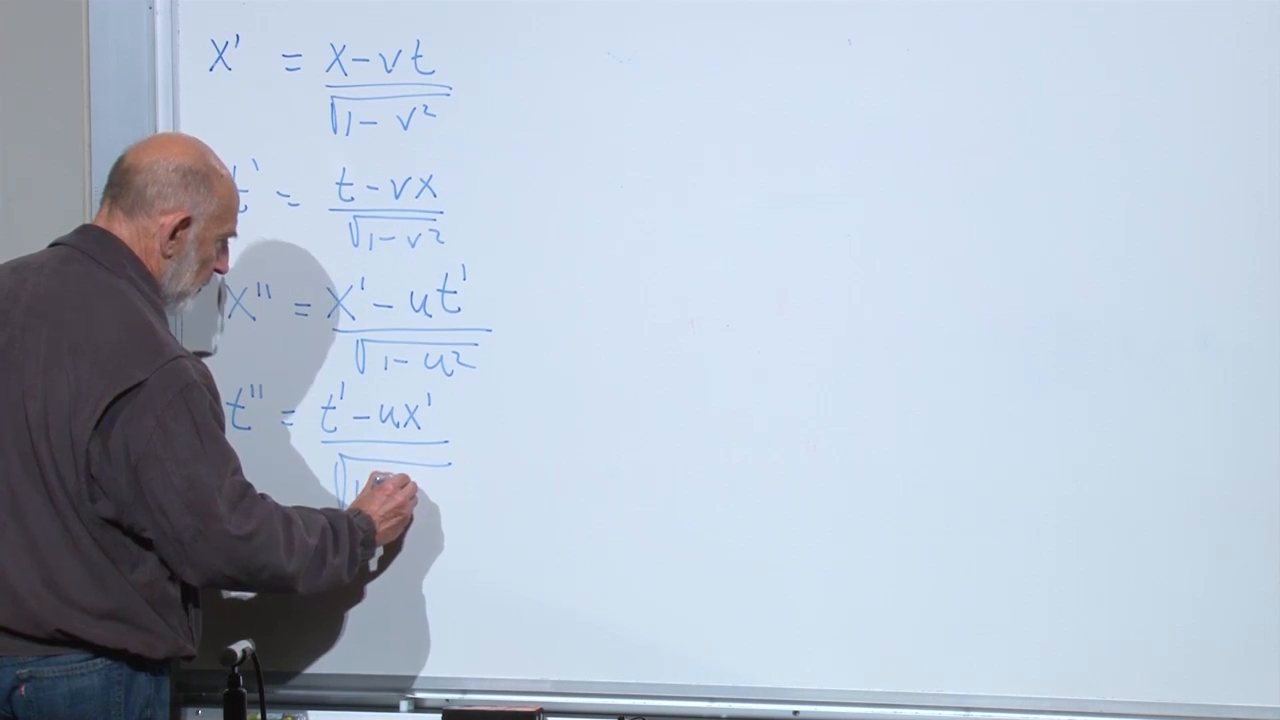
\includegraphics[width=0.90\textwidth]{lecture_02_figure_03.png}
\caption{从车站到列车的正变换公式之后，是第二个从带撇坐标到双撇坐标的洛伦兹变换。}
\lectureframe{00:14:55}
\end{figure}

\subsection{将一个推促代入另一个}

空间方程足以求出\(w\)。将\eqref{eq:sr2-direct}代入\eqref{eq:sr2-second-boost}的第一个方程：
\begin{align}
x''
&=\gamma_u(x'-ut')\\
&=\gamma_u\gamma_v\left[(x-vt)-u(t-vx)\right]\\
&=\gamma_u\gamma_v\left[(1+uv)x-(u+v)t\right].
\label{eq:sr2-composed-space}
\end{align}
\(uvx\)项中的两个负号使它变为正；两个时间项合并为\(-(u+v)t\)。

\begin{figure}[htbp]
\centering
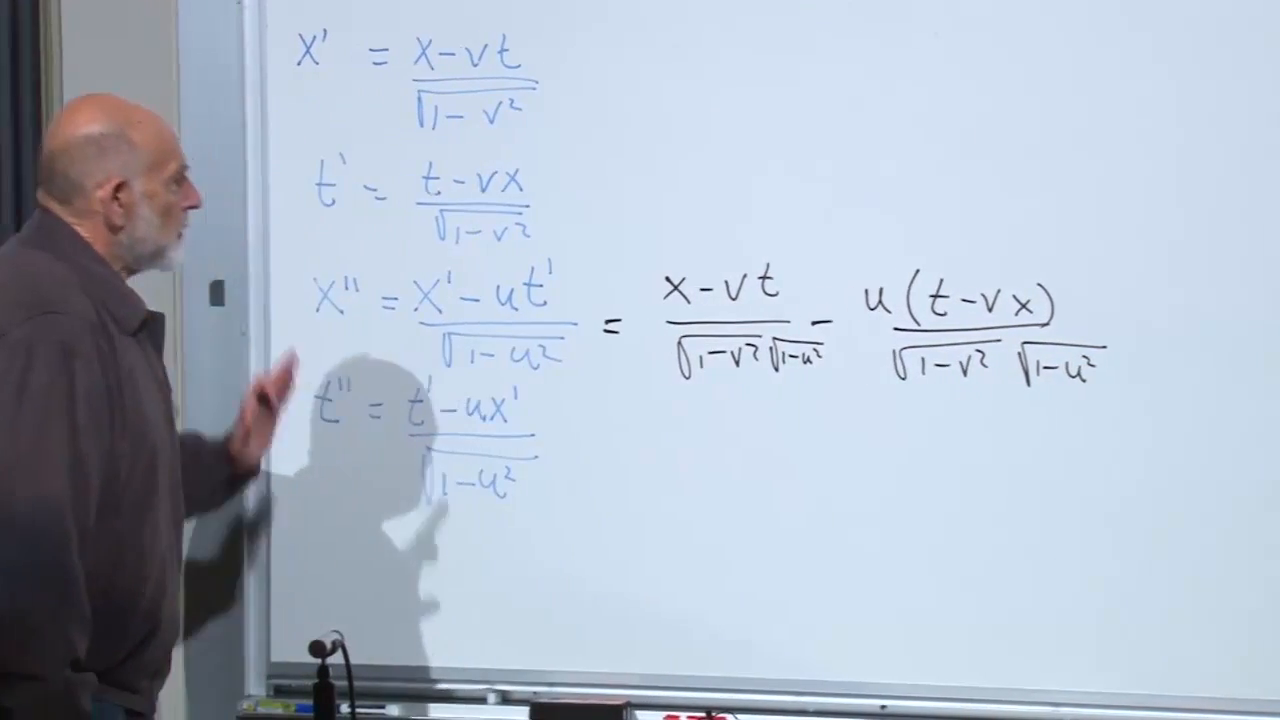
\includegraphics[width=0.91\textwidth]{lecture_02_figure_04.png}
\caption{在合成推促中收集\(x\)项和\(t\)项之前的嵌套代入。}
\lectureframe{00:16:30}
\end{figure}

和之前一样，在确定运动原点时，分母无关紧要。童车在\(x''=0\)处静止，所以\eqref{eq:sr2-composed-space}中的括号必须为零：
\begin{equation}
(1+uv)x-(u+v)t=0.
\end{equation}
因此它在车站参考系中的世界线为
\begin{equation}
x=\frac{u+v}{1+uv}\,t,
\end{equation}
而其速度为
\begin{equation}
\boxed{w=\frac{u+v}{1+uv}}.
\label{eq:sr2-velocity-add-c1}
\end{equation}

\begin{figure}[htbp]
\centering
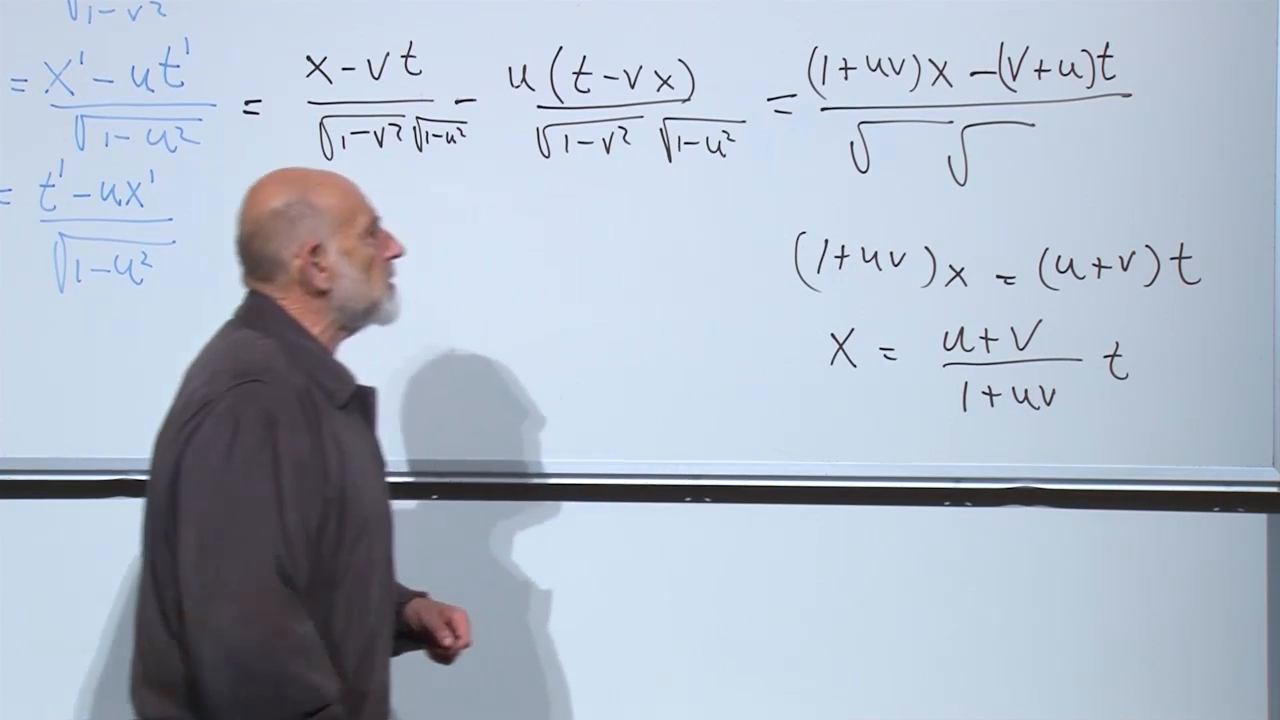
\includegraphics[width=0.91\textwidth]{lecture_02_figure_05.png}
\caption{收集后的分子与世界线\(x=[(u+v)/(1+uv)]t\)揭示了合成速度。}
\lectureframe{00:19:30}
\end{figure}

时间方程也一致地合成。从车站到童车的完整变换具有洛伦兹形式
\begin{align}
x''&=\gamma_w(x-wt),&
t''&=\gamma_w(t-wx),
\end{align}
其中
\begin{equation}
\gamma_w=\frac{1}{\sqrt{1-w^2}}.
\end{equation}
确实，
\begin{equation}
\gamma_w=\gamma_u\gamma_v(1+uv),
\end{equation}
这可以通过代入\eqref{eq:sr2-velocity-add-c1}并化简得到。因此，两个共线推促合成为另一个共线推促。

\subsection{恢复量纲}

\begin{classroomqa}
\audiencequestion{为什么在普通单位中分母\(1+uv\)在量纲上不正确？}
\lecturerresponse{它之所以正确，只是因为\(c=1\)使每个速度都成为光速的无量纲分数。在常规单位中，该乘积必须表现为\(uv/c^2\)，这是无量纲的。\lecturetimestamp{00:21:11}}
\end{classroomqa}

具有量纲的速度相加定律为
\begin{equation}
\boxed{
w=\frac{u+v}{1+\dfrac{uv}{c^2}}
}.
\label{eq:sr2-velocity-add}
\end{equation}

\begin{figure}[htbp]
\centering
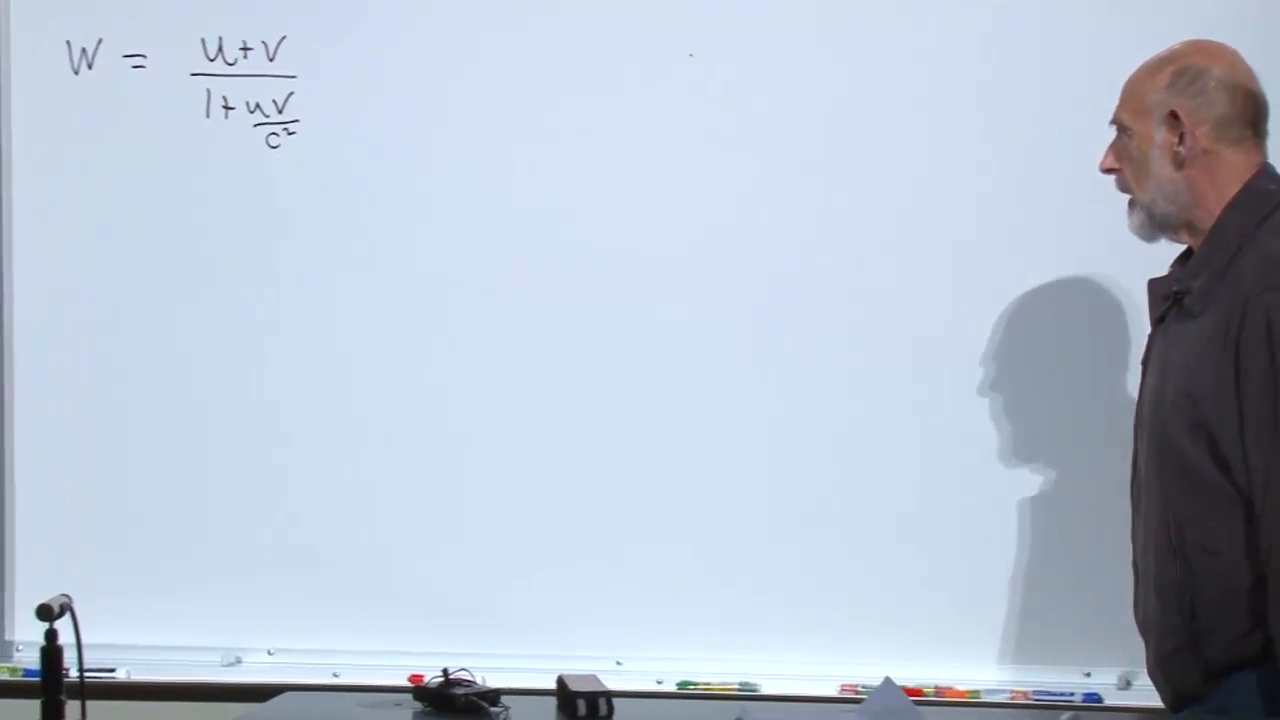
\includegraphics[width=0.90\textwidth]{lecture_02_figure_06.png}
\caption{量纲一致性在乘积\(uv\)之下恢复了\(c^2\)。}
\lectureframe{00:22:06}
\end{figure}

对于\(\lvert u\rvert,\lvert v\rvert\ll c\)，
\begin{equation}
\frac{uv}{c^2}\ll 1,
\end{equation}
因此
\begin{equation}
w\approx u+v.
\end{equation}
牛顿式相加是低速近似，而不是一条独立的规则。

\subsection{两种数值情形}

首先取
\begin{equation}
u=v=0.01c.
\end{equation}
在单位\(c=1\)下，
\begin{equation}
w=\frac{0.02}{1.0001}\approx 0.019998.
\end{equation}
光速的百分之一已经约为\(3\times10^6\ {\rm m/s}\)，然而相对论修正却只有万分之一。结果略小于牛顿式的\(0.02c\)。

\begin{figure}[htbp]
\centering
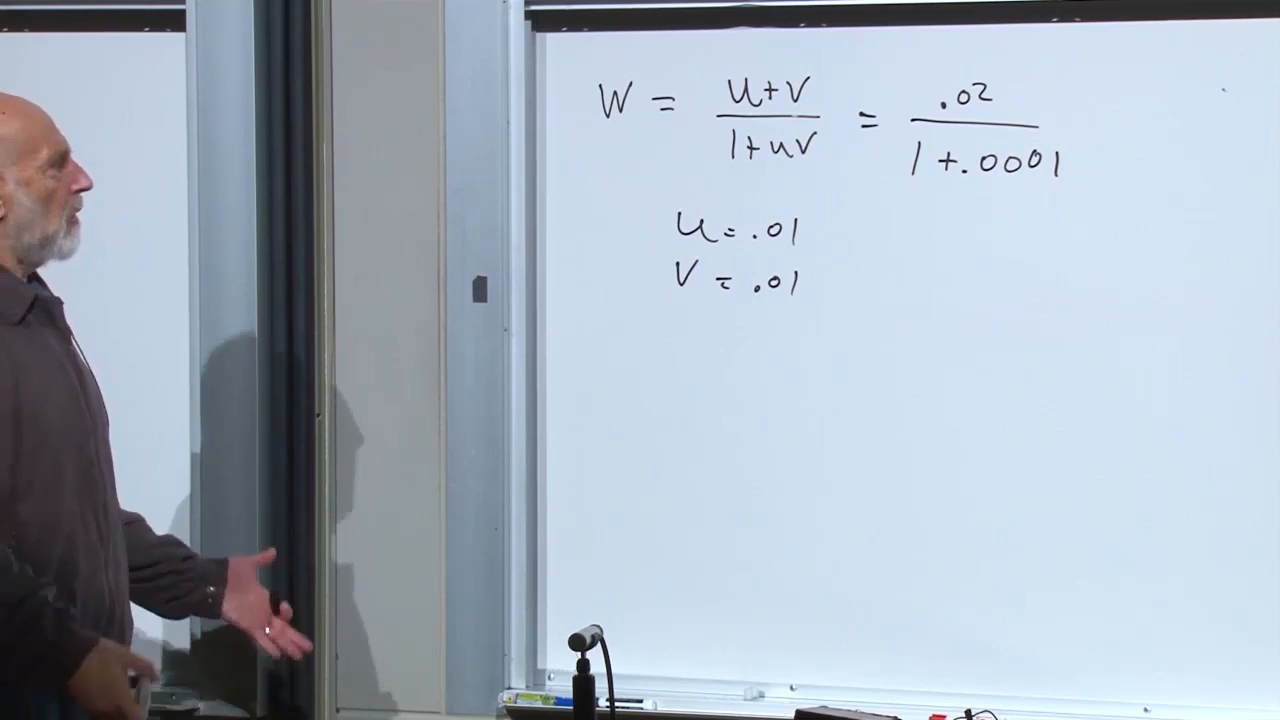
\includegraphics[width=0.90\textwidth]{lecture_02_figure_07.png}
\caption{在\(u=v=0.01c\)处，分母与1的差别仅为\(10^{-4}\)。}
\lectureframe{00:24:23}
\end{figure}

现在取
\begin{equation}
u=v=0.9c.
\end{equation}
牛顿会预言\(1.8c\)。相对论给出
\begin{equation}
\frac{w}{c}
=\frac{0.9+0.9}{1+0.9^2}
=\frac{1.8}{1.81}
\approx 0.9945.
\label{eq:sr2-fast-example}
\end{equation}

\begin{figure}[htbp]
\centering
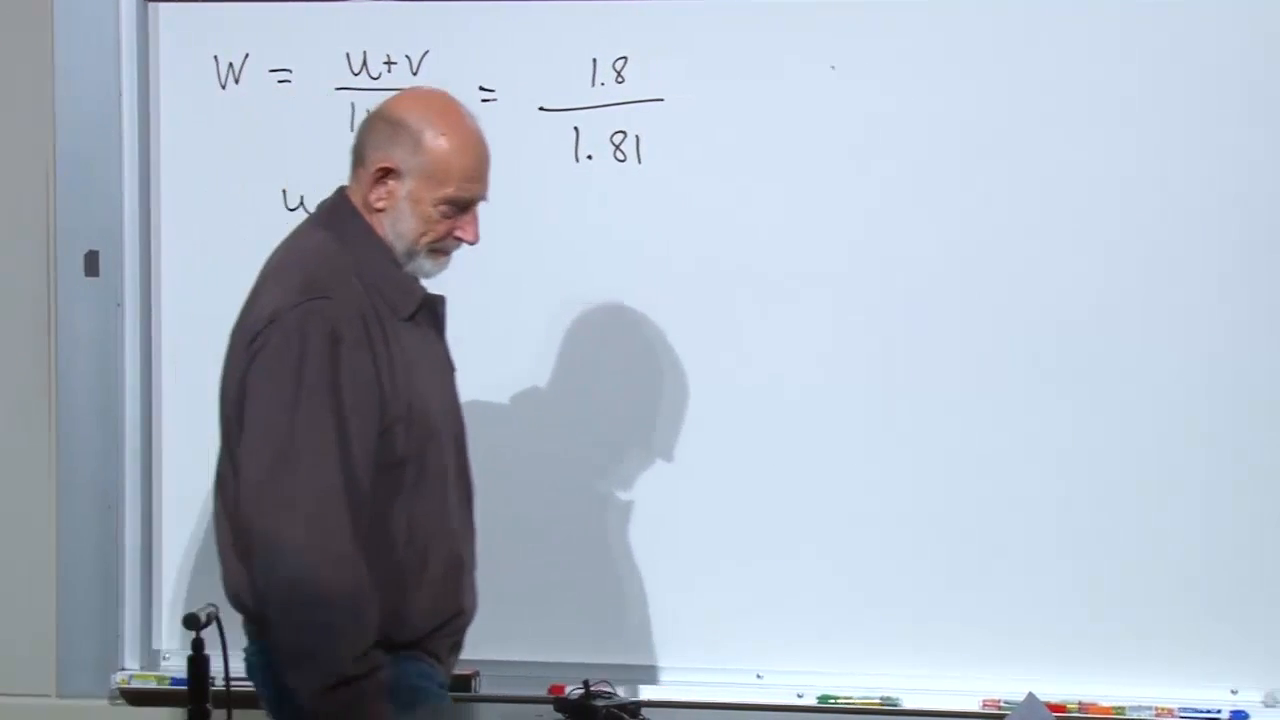
\includegraphics[width=0.90\textwidth]{lecture_02_figure_08.png}
\caption{两个\(0.9c\)的速度合成为\(1.8/1.81\)，仍然低于光速。}
\lectureframe{00:25:48}
\end{figure}

相继的亚光速推动不能越过\(c\)。若\(u<c\)且\(v<c\)，则
\begin{equation}
1-\frac{w}{c}
=
\frac{\left(1-\frac{u}{c}\right)
      \left(1-\frac{v}{c}\right)}
     {1+\frac{uv}{c^2}}
>0.
\end{equation}
每一次额外的推动都能使结果更接近\(c\)，但永远不会超过它。在极限值\(u=c\)处，
\begin{equation}
w=\frac{c+v}{1+v/c}=c.
\end{equation}
光速是合成定律的一个不动点。

\section{坐标测量并非视觉外观}

\begin{classroomqa}
\audiencequestion{如果列车有玻璃墙，车站观察者能否只是同时看着乘客和小童车，并直接读出它们的运动？}
\lecturerresponse{洛伦兹变换涉及用分布各处的直尺和同步时钟所作的坐标测量。视觉图像还包含来自不同事件的光到达观察者的不相等传播时间。玻璃改变的是所见景象，而不是坐标关系；把一幅图像当作同时的数据，会重新引入相对论所纠正的那个同时性假设。\lecturetimestamp{00:27:53}}
\end{classroomqa}

一个事件在每个参考系中都有位置和时间，无论是否恰好有人在那时看到它。光学外观是一个正当的主题，但它需要第二次计算，追踪光从每个事件到眼睛的路径。变换定律本身是普适的，与列车墙壁无关。

\section{三维空间中的固有间隔}

回到两个事件，起初一个位于原点，另一个位于\((x,t)\)。在一维空间中，
\begin{equation}
\tau^2=t^2-x^2
\label{eq:sr2-interval-1d}
\end{equation}
在单位\(c=1\)下。每个惯性系都同意：
\begin{equation}
\tau^2
=t^2-x^2
=t'^2-x'^2
=t''^2-x''^2.
\end{equation}
坐标改变；固有间隔不变。

对于类时间隔，一个时钟可以在两个事件之间运动。如果它在第一个事件处读数为正午，那么它在第二个事件处的经过读数就是固有时间\(\tau\)。这一陈述与用哪个坐标参考系来计算间隔无关。

\begin{figure}[htbp]
\centering
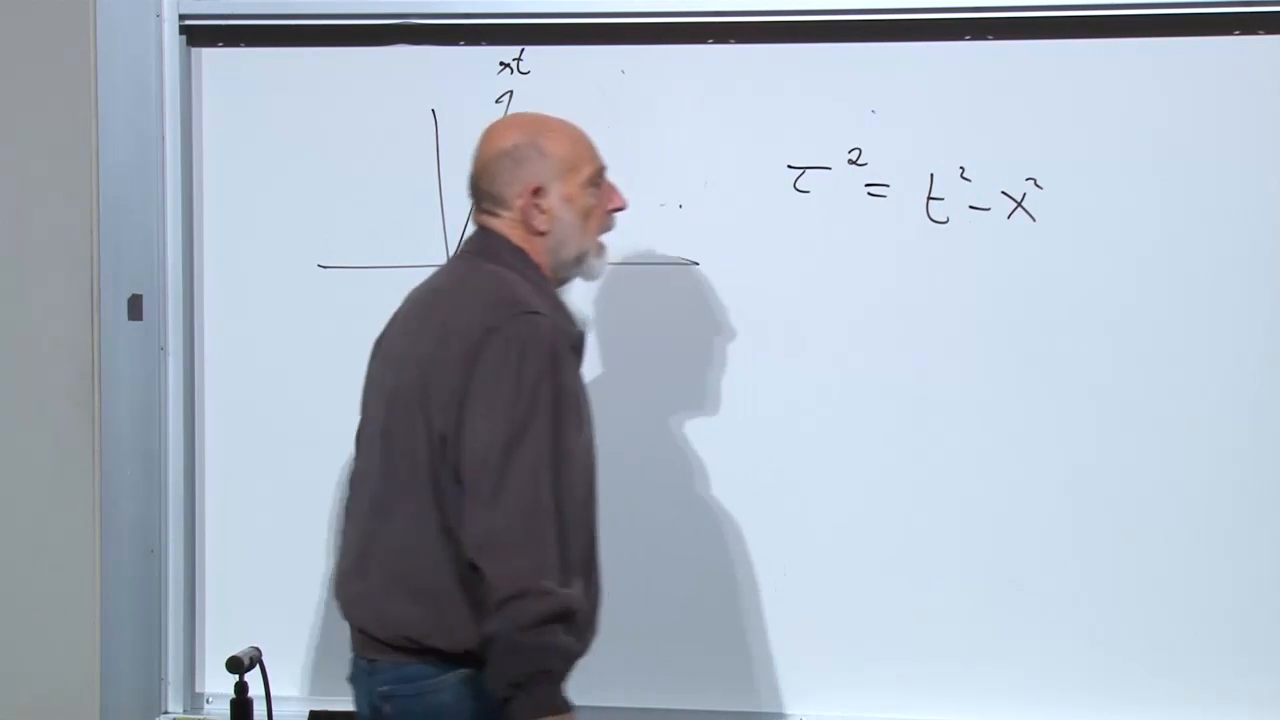
\includegraphics[width=0.90\textwidth]{lecture_02_figure_09.png}
\caption{在恢复横向方向之前，先回顾不变固有时间关系\(\tau^2=t^2-x^2\)。}
\lectureframe{00:30:18}
\end{figure}

\subsection{空间旋转恢复横向方向}

在回到推动之前，考虑空间坐标轴的普通旋转。一个不位于\(x\)轴上的点，其空间距离平方为
\begin{equation}
r^2=x^2+y^2+z^2,
\end{equation}
根据普通的毕达哥拉斯定理，它在旋转下不变。因此，\(3+1\)维时空间隔为
\begin{equation}
\boxed{
\tau^2=t^2-x^2-y^2-z^2
}.
\label{eq:sr2-interval-3d}
\end{equation}
恢复\(c\)后，
\begin{equation}
c^2\tau^2
=c^2t^2-x^2-y^2-z^2.
\end{equation}

\begin{figure}[htbp]
\centering
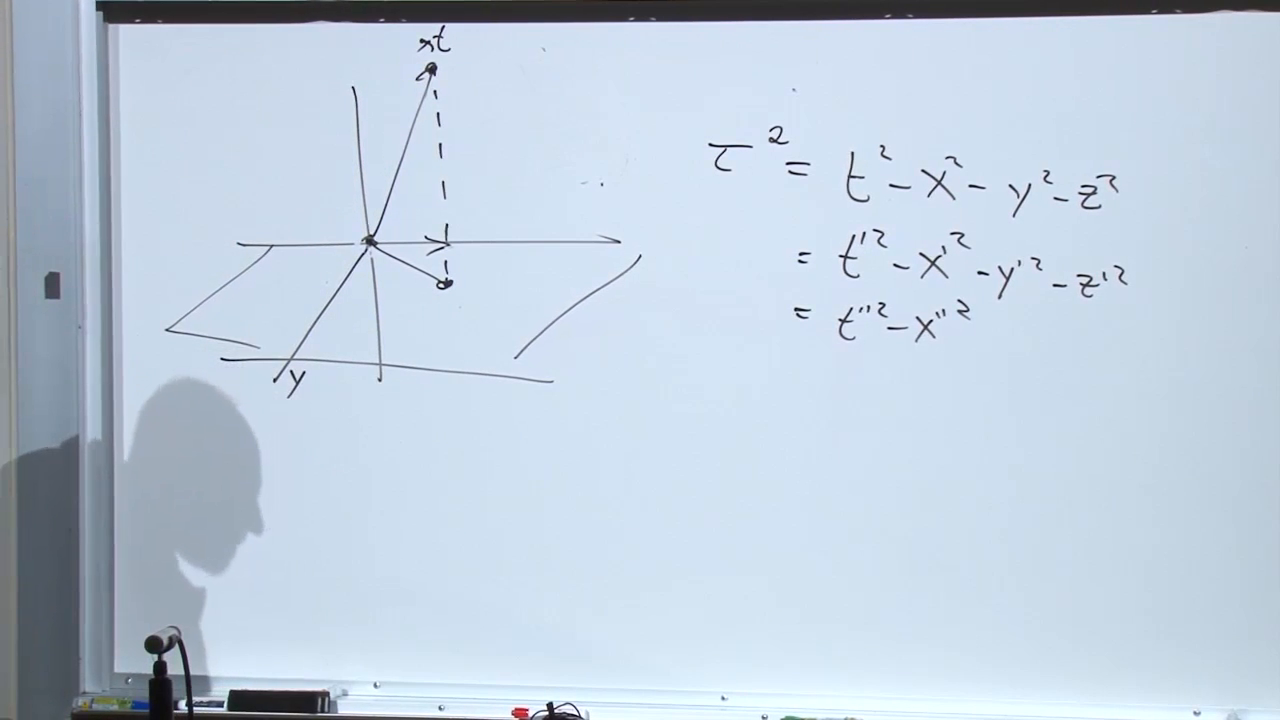
\includegraphics[width=0.90\textwidth]{lecture_02_figure_10.png}
\caption{毕达哥拉斯空间距离把不变量从\(t^2-x^2\)推广到\(t^2-x^2-y^2-z^2\)。}
\lectureframe{00:34:23}
\end{figure}

空间旋转与洛伦兹推动的任意组合都保持\eqref{eq:sr2-interval-3d}。普通的坐标轴对分量有分歧，但对欧几里得距离一致；惯性时空参考系对空间和时间分量有分歧，但对这个平方差一致。该不变量是狭义相对论的核心几何事实。

\begin{classroomqa}
\audiencequestion{如果乘客把小童车换成一束向前的闪光灯，列车观察者和车站观察者会得到相同的光速吗？}
\lecturerresponse{在\eqref{eq:sr2-velocity-add}中令\(u=c\)。于是\(w=(c+v)/(1+v/c)=c\)。在\(c=1\)单位下，该比值就是\((1+v)/(1+v)=1\)。两个参考系测得相同的速率，完全符合要求。\lecturetimestamp{00:35:53}}
\end{classroomqa}

因此，先前关于玻璃墙的担忧并不是不变光速的失败。它是把坐标测量与延迟的视觉图像混为一谈，归根结底是把同时性弄混了。

\section{零射线与光锥}

在一维空间中，向右和向左运动的光线满足
\begin{equation}
x=\pm t.
\end{equation}
它们的间隔为零：
\begin{equation}
t^2-x^2=0.
\end{equation}
与欧几里得距离不同，零时空间隔并不要求事件重合。它意味着一个光信号能够连接它们。

当所有空间方向都被恢复后，光线满足
\begin{equation}
t^2-x^2-y^2-z^2=0,
\label{eq:sr2-null}
\end{equation}
或
\begin{equation}
r=t
\end{equation}
其中在\(c=1\)单位制下，光指向未来。

\begin{figure}[htbp]
\centering
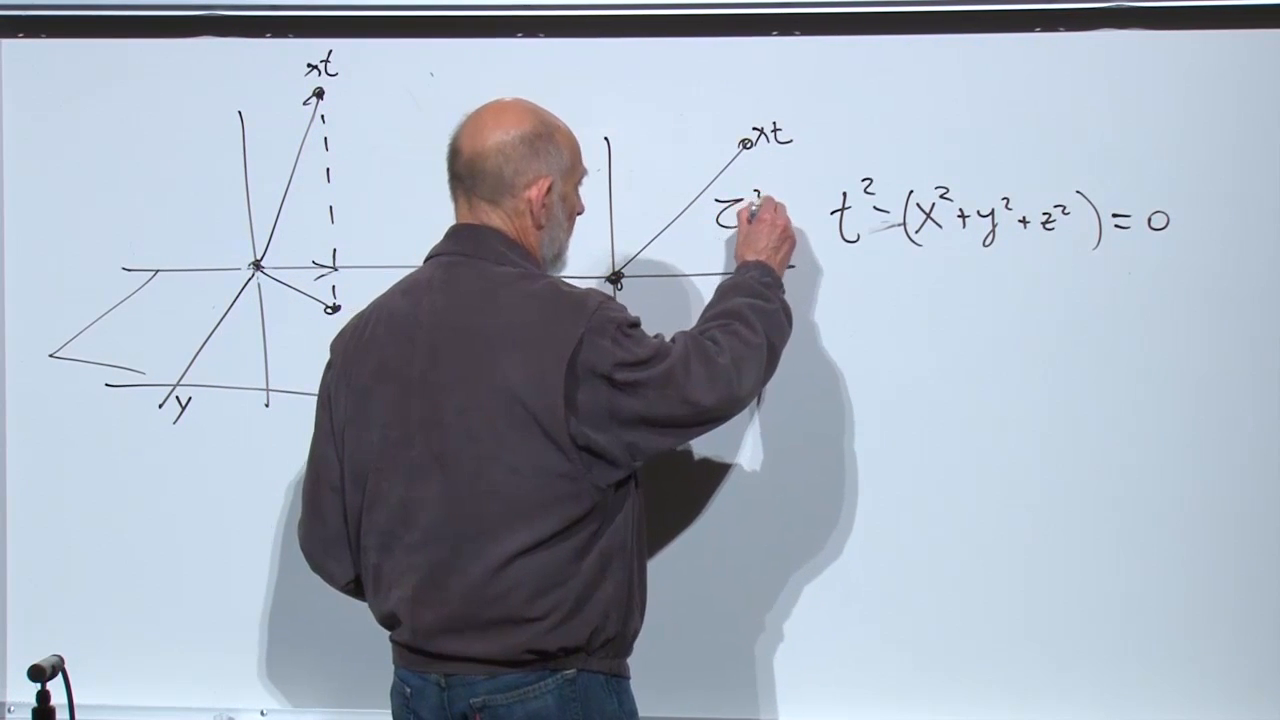
\includegraphics[width=0.90\textwidth]{lecture_02_figure_11.png}
\caption{任意空间方向上的光都遵循满足\(t^2-(x^2+y^2+z^2)=0\)的零轨迹。}
\lectureframe{00:39:28}
\end{figure}

在\(1+1\)维中，零集是一对\(45^\circ\)线。当有两个空间维度加时间时，它变成一个锥；三个空间维度无法在板上完整显示，但定义方程不变。

未来光锥由原点发出的光能够到达的事件组成。过去光锥由光能够到达原点的事件组成。一个是另一个在时间上翻转。

\begin{figure}[htbp]
\centering
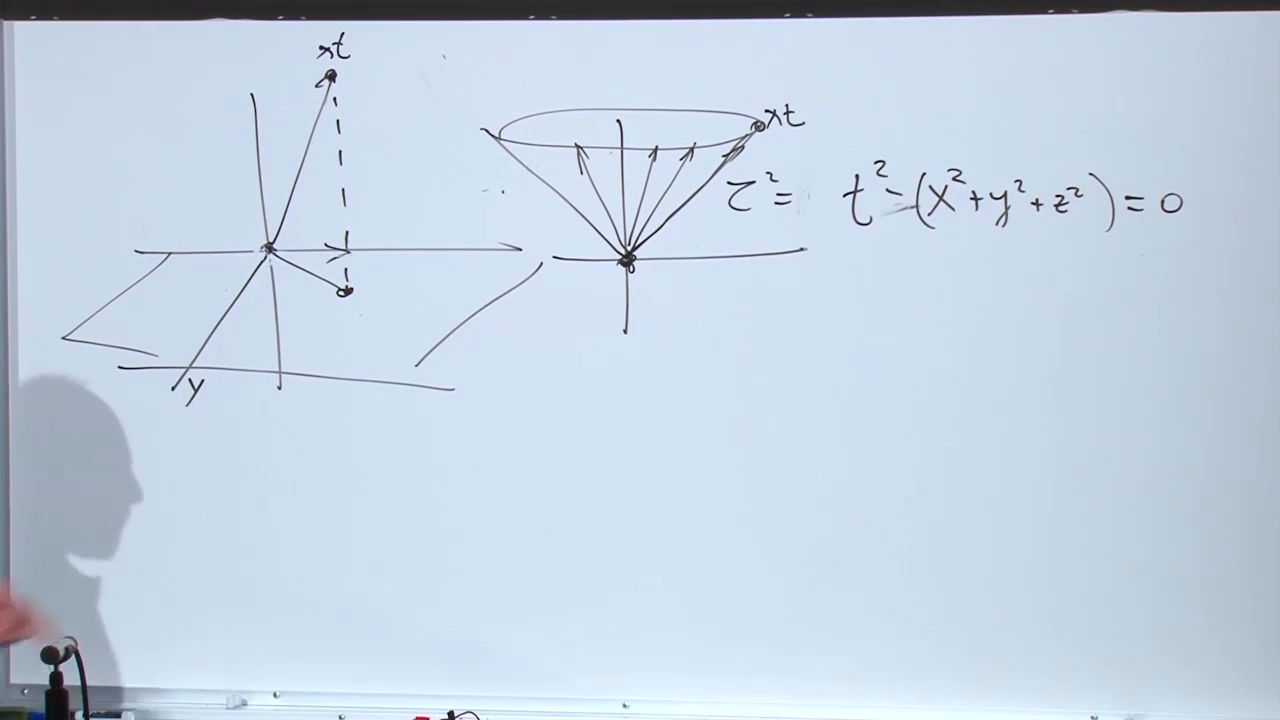
\includegraphics[width=0.90\textwidth]{lecture_02_figure_12.png}
\caption{在更高维时空图中，\(45^\circ\)零光线扫出未来光锥和过去光锥。}
\lectureframe{00:40:47}
\end{figure}

\begin{classroomqa}
\audiencequestion{在牛顿力学中，伽利略变换下对应的不变量是什么？}
\lecturerresponse{时间间隔本身。牛顿观察者都同意\(\Delta t\)，尽管他们对空间位移有分歧。相对论放弃了普遍时间，并用不变时空间隔取而代之。\lecturetimestamp{00:41:53}}
\end{classroomqa}

\section{从空间矢量到四维矢量}

这里的矢量是几何矢量，不是量子态矢量。普通空间中两点之间的位移具有大小和方向。它的尾端可以平移到原点而不改变矢量，其三个分量可以记为
\begin{equation}
x^i=(x^1,x^2,x^3)=(x,y,z),
\qquad i=1,2,3.
\end{equation}
拉丁指标\(i\)只遍历空间方向。

一个事件还需要一个额外分量，即它的时间。因此时空位置写作
\begin{equation}
x^\mu=(x^0,x^1,x^2,x^3)=(t,x,y,z),
\qquad \mu=0,1,2,3.
\label{eq:sr2-four-position}
\end{equation}
按照历史惯例，时间是第零个分量而不是第四个：
\begin{equation}
x^0=t,\qquad x^1=x,\qquad x^2=y,\qquad x^3=z.
\end{equation}
希腊指标如\(\mu\)遍历时空；拉丁指标如\(i\)遍历空间。

\begin{figure}[htbp]
\centering
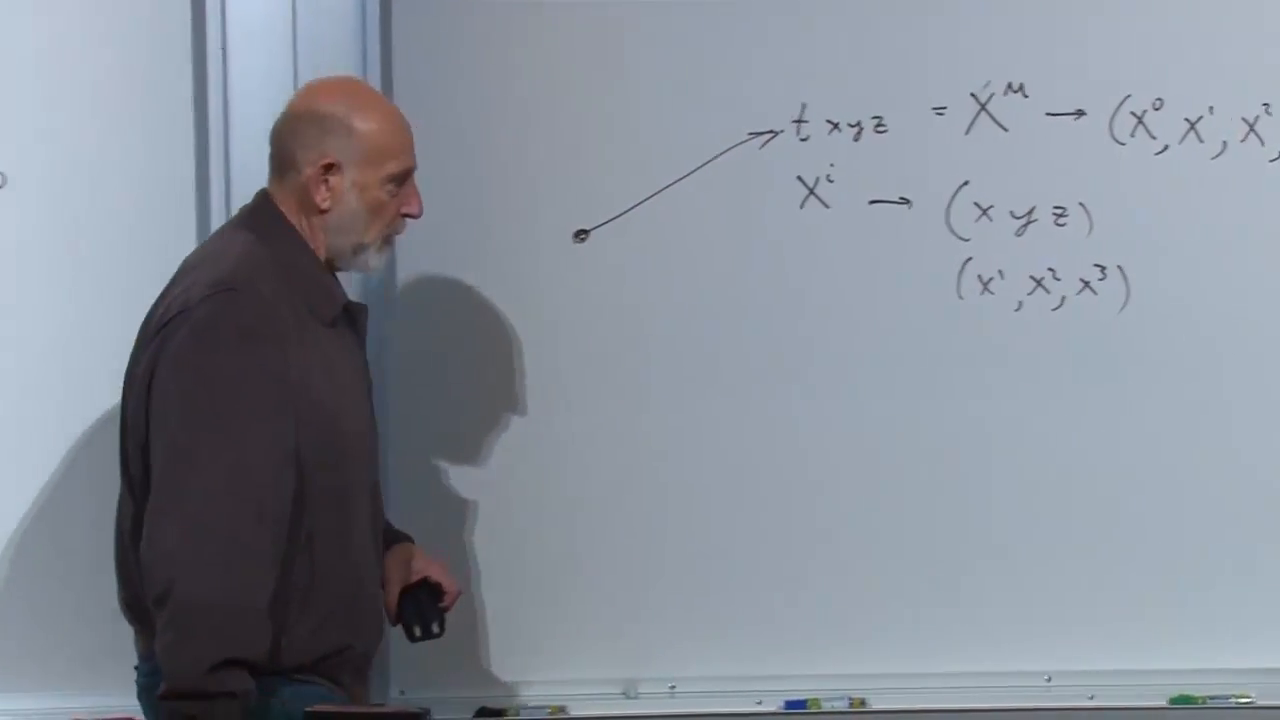
\includegraphics[width=0.90\textwidth]{lecture_02_figure_13.png}
\caption{空间分量\(x^i\)被扩充为四分量时空位置\(x^\mu=(x^0,x^1,x^2,x^3)\)。}
\lectureframe{00:46:05}
\end{figure}

不变量变为
\begin{equation}
\tau^2
=(x^0)^2-(x^1)^2-(x^2)^2-(x^3)^2.
\end{equation}
仅凭记号并不增加新的物理内容。其价值在于洛伦兹变换线性地作用于所有四个分量，正如旋转线性地作用于空间矢量。

\begin{classroomqa}
\audiencequestion{既然变换是线性的，它能否用作用于列矢量的矩阵来表示？}
\lecturerresponse{可以。对于沿\(x\)方向的助推，非平凡块是作用于\((t,x)^{\mathsf T}\)的\(\gamma_v\begin{pmatrix}1&-v\\-v&1\end{pmatrix}\)，而\(y\)和\(z\)不变。矩阵记号是组合和组织洛伦兹变换的自然方式。\lecturetimestamp{00:48:14}}
\end{classroomqa}

显式地，
\begin{equation}
\begin{pmatrix}
t'\\x'\\y'\\z'
\end{pmatrix}
=
\begin{pmatrix}
\gamma_v&-\gamma_v v&0&0\\
-\gamma_v v&\gamma_v&0&0\\
0&0&1&0\\
0&0&0&1
\end{pmatrix}
\begin{pmatrix}
t\\x\\y\\z
\end{pmatrix}.
\label{eq:sr2-boost-matrix}
\end{equation}

\section{位移与四维速度}

从一个事件的位置移动到粒子世界线的一小段。四维位移是
\begin{equation}
\Delta x^\mu
=(\Delta t,\Delta x,\Delta y,\Delta z).
\end{equation}
当位移被称为小时，微积分正在逼近：\(\Delta x^\mu\)将变为\(dx^\mu\)。目前，有限记号使几何变得透明。

沿类时世界线的固有时增量满足
\begin{equation}
(\Delta\tau)^2
=(\Delta t)^2-(\Delta x)^2-(\Delta y)^2-(\Delta z)^2.
\label{eq:sr2-proper-increment}
\end{equation}
普通速度用坐标时间除空间位移，并具有三个分量。四维速度则用不变固有时除四维位移：
\begin{equation}
u^\mu
=\frac{\Delta x^\mu}{\Delta\tau}
\quad\longrightarrow\quad
\boxed{
u^\mu=\frac{dx^\mu}{d\tau}
}.
\label{eq:sr2-four-velocity}
\end{equation}

\begin{figure}[htbp]
\centering
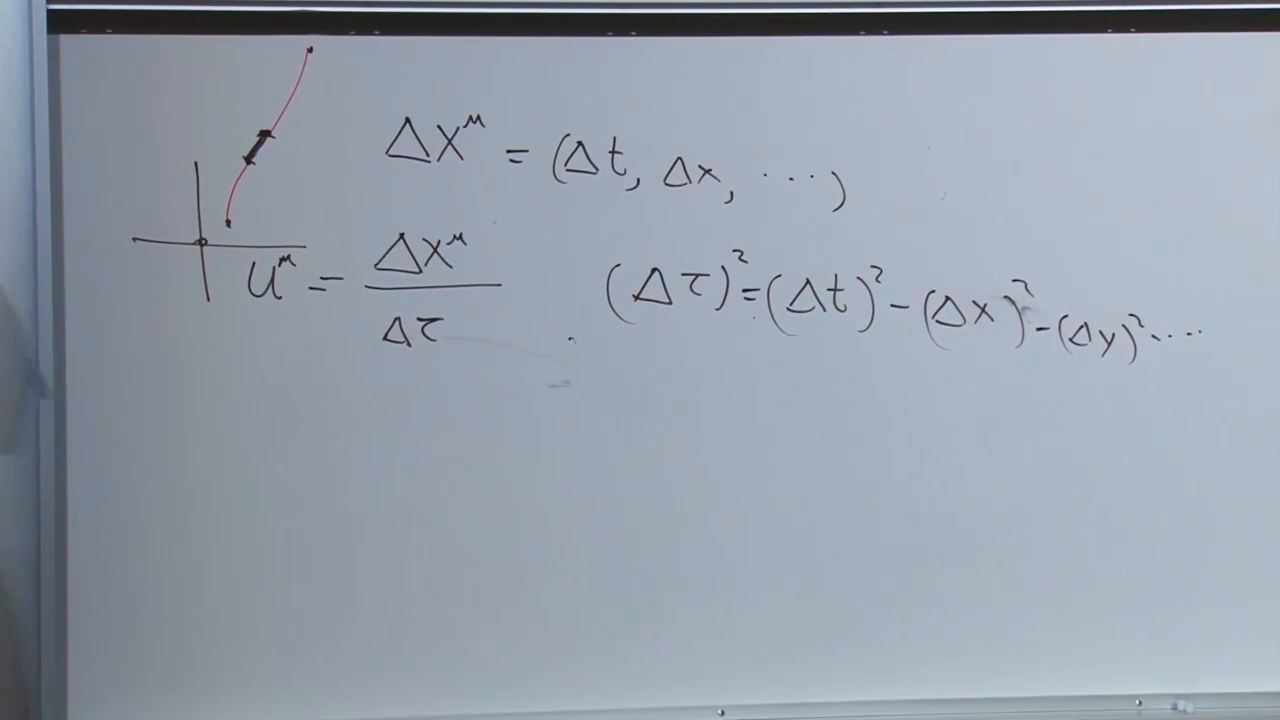
\includegraphics[width=0.90\textwidth]{lecture_02_figure_14.png}
\caption{一段世界线定义了\(\Delta x^\mu\)、其不变量\(\Delta\tau\)以及四维速度\(u^\mu=\Delta x^\mu/\Delta\tau\)。}
\lectureframe{00:52:42}
\end{figure}

这个对象有四个分量，并像四维矢量一样变换。它与普通三维速度的关系是下一个问题，此处有意留待解决。解决它将引向相对论动量、能量、加速度，并最终引向\(F=ma\)的相对论推广。
